
\section{Fundamental Groups}
We now depart the world of combinatorial topology for a little bit to describe the fundamental group. The Fundamental group was developed in the late 19th century by \cite{poincare1895analysis}, and is usually the first tool that one learns in algebraic topology. We've placed the fundamental group at the end of this course as a transition point between the study of combinatorial methods in topology and the full modern theory of algebraic topology. \\
Informally, the fundamental group provides an algebraic framework for understanding the paths that one can draw on a space. Since one can draw infinitely many different paths on a space, we restrict our attention to loops with a fixed start / endpoint, and we only consider equivalence classes of paths up to the relation of homotopy.\\
With these restrictions, the set of paths that exist becomes a lot more manageable. Here are two examples to keep in mind going forward:
\examplefigure[Paths on Disks]{
	On the Disk, there is only 1 equivalence class of such paths, as they all may be deformed to a point. }{Disk with Contracting Loop}
\examplefigure[Paths on Circles]{
	On a circle, the equivalence classes of such paths is in bijection with the integers. If two paths $\gamma_1$ and $\gamma_2$ have the same winding number around the circle, we know that we can deform one path into the other.  }{Loops on circles}
After a quick overview of some of the topological properties of the fundamental group, we'll give some combinatorial methods for computing the fundamental group, and use intuition from the fundamental group to better our understanding of knots.\\
In order to continue, we'll assume the reader has some familiarity with topological spaces and continuity from point-set topology. Our exposition of the fundamental group will be very brief, primarily designed to get the reader up to speed with conventions and notations so we can look at applications of the fundamental group to knot theory. A student hoping to get a well-grounded foundation in fundamental groups and homotopy is encouraged to read a more substantiative text like \cite{hatcher2002algebraic}. 
\begin{doubledtuftepage}[Paths and Homotopy Equivalence]

\begin{definition} Let $X$ be a topological space,  and $x_0,  x_1\in X$ be two points. A \emph{path} in $X$ with endpoints $p$ and $q$ is a continuous function $\gamma: [0, 1]\to X$ with the property that $\gamma(0)=p$ and $\gamma(1)=q$. If $p=q$,  we say that $\gamma$ is a \emph{loop},  and we call $x_0$ the \emph{base point} of those loops. 
\end{definition}

\begin{definition}
	 \smarginnote{	\begin{align*}
		H(x,  0)=&f_0(x)\\
		H(x,  1)=&f_1(x).
		\end{align*}}
	Let $f_0:X\to Y$ and $f_1: X\to Y$ be two different functions. A \emph{homotopy} between $f_0$ and $f_1$ is a continuous function $H(x,  t):X\times [0,1]\to Y$ whose restriction to the boundaries match $f_i$. 
	If there is a homotopy between $f_0$ and $f_1$,  we say that $f_0$ is \emph{homotopic} to $f_1$ and write $f_0\sim f_1$.
\end{definition}
Homotopy tells us when two maps between topological spaces are equivalent under a parameterized deformation. Since we think of loops as functions into our target space, we can use the above definition to describe deformation equivalent loops. 
\begin{definition}\smarginnote{\begin{align*}
		H(0, t)=&p\\
		H(1, t)=&q.
		\end{align*}}
	Let $X$ be a topological space  and $\gamma_0$ nd $\gamma_1$ be two paths with matching left and right endpoints  $p,  q\in X$.	 Then a \emph{path homotopy from $\gamma_0$ to $\gamma_1$} is a homotopy between $\gamma_0$ and $\gamma_1$ which always agrees on the endpoints. In this case, we write $\gamma_0\sim \gamma_1$ and say that they are \emph{homotopic.} 
\end{definition}
The notion of path homotopy is more restrictive than homotopy, as the endpoints of the paths are required to be fixed\footnote{Notice, for example, if the space $X$ is path connected, then all paths are homotopic, but not necessarily path homotopic. (Exercise \ref{exer:homotopicvspathhomotopic})}. We will work with homotopies of paths so often that it'll be useful to have a diagrammatic representation of homotopies. \smarginnote{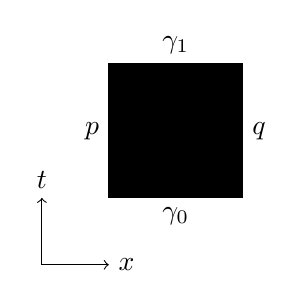
\begin{tikzpicture}[scale=.85]
	\draw[fill=\shadinga] (0, 0) rectangle (2, 2);
	\draw (1,1) node {$H_{01}$};
	\draw (1, 0) node[below] {$\gamma_0$};
	\draw (0, 1) node[left] {$p$};
	\draw (1, 2) node[above] {$\gamma_1$};
	\draw (2,  1) node[right] {$q$};	
	\draw[->] (-1, -1)--(-1, 0) ;
	\draw[->] (-1, -1)--(0,-1);
	\draw (-1,  0) node[above] {$t$};
	\draw (0, -1) node[right] {$x$};
	\end{tikzpicture}}
Notice that a homotopy between paths is nothing more than a map between $[0,1]\times [0,1]\to X$, where coordinate gives the homotopy parameter $t$ and the other one represents the path parameter $x$. The left and right portions of the square are mapped to the mutual endpoints of $\gamma_i$, and the top and bottom edges are the maps $\gamma_i$. \\

\begin{claim}
	Path homotopy is an equivalence relation on paths from $p$ to $q$. For each equivalence class of paths, we will write $[\gamma]$, the \emph{homotopy class of $\gamma$}
\end{claim}
\begin{proof}
We'll need to check the three properties of an equivalence relation. In order to do this, we'll have to construct homotopies between paths, and this proof serves as an introduction to the intuition afforded by the diagrammatic representation of path homotopies. \\
\smarginnotel{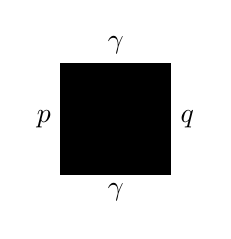
\begin{tikzpicture}[scale=.7]
	\draw[fill=\shadinga] (0, 0) rectangle (2, 2);
	\draw (1, 0) node[below] {$\gamma$};
	\draw (0, 1) node[left] {$p$};
	\draw (1, 2) node[above] {$\gamma$};
	\draw (2,  1) node[right] {$q$};	
	\draw[dashed] (0, .3)--(2, .3);
	\draw (1, .3) node[above] {$\gamma$};
	\end{tikzpicture}}We first need to show that the relation is \emph{reflexive.}
Let $\gamma_0: I\to X$ be any path. We can define the constant homotopy $H(x,  t)=\gamma(x)$ for all $t$, which is a homotopy between $\gamma$ and itself. In the diagram in the right, the dashed line and label indicates that the homotopy restricted to the dashed line gives us the path $\gamma$ in $X$.  \\

Next, we'll check that the relation of homotopy is \emph{symmetric.} \smarginnotel{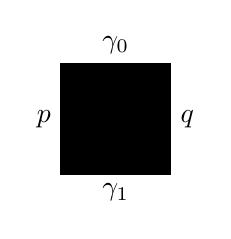
\begin{tikzpicture}[scale=.7]
	\draw[fill=\shadinga] (0, 0) rectangle (2, 2);
	\draw (1, 0) node[below] {$\gamma_1$};
	\draw (0, 1) node[left] {$p$};
	\draw (1, 2) node[above] {$\gamma_0$};
	\draw (2,  1) node[right] {$q$};
	\draw (1,1) node {\scalebox{1}[-1]{$H_{01}$}};
	\end{tikzpicture}} Suppose that $H_{01}(x,  t)$ is a homotopy between $\gamma_0$ and $\gamma_1$. Then we can define the \emph{reverse homotopy} \[H_{10}(x, t):=(x, 1-t)\] which is a homotopy between $\gamma_1$ and $\gamma_0$. In the diagram, the reflected text is suppose to tell us that the domain of the homotopy has been precomposed with a reflection map. \\

Finally, we need to check\emph{ transitivity.}\smarginnotel{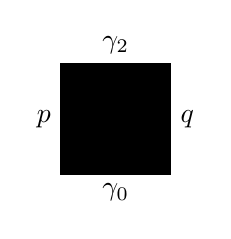
\begin{tikzpicture}[scale=.7]
	\draw[fill=\shadinga] (0, 0) rectangle (2, 2);
	\draw (1, 0) node[below] {$\gamma_0$};
	\draw (0, 1) node[left] {$p$};
	\draw (1, 2) node[above] {$\gamma_2$};
	\draw[dashed] (0,1) -- (2,1);
	\draw (2,  1) node[right] {$q$};
	\draw (1, .5) node {$H_{01}$};
	\draw (1, 1.5) node {$H_{12}$};
	\end{tikzpicture}} Suppose that $H_{01}(x,  t)$ is a homotopy between $\gamma_0$ and $\gamma_1$,  and $H_{12}(x,  t)$ is a homotopy between $\gamma_1$ and $\gamma_2$. Then define a new homotopy $H_{02}$ by 
		\[
			H_{02}(x,  t)=\left\{\begin{array}{cc}
			                     	H_{01}(x, 2t) & t\in [0, 1/2]\\
			                     	H_{12}(x, 2t-1) & t\in (1/2,  1]
			                     \end{array}\right. .
		\]
		You should check that this gives us an honest continuous homotopy between $\gamma_0$ and $\gamma_1$. In the diagram on the right, we see that our new homotopy is constructed by gluing together the domains of our old homotopies together. 

\end{proof}


\end{doubledtuftepage}

\begin{doubledtuftepage}[Concatenation and Homotopy]
We'll now look at how we can assemble loops together on a space. Given two loops, we can create a new loop which goes through each of the original loops at double speed. 
\begin{definition}
	Let $\gamma_0,  \gamma_1$ be two loops with base point $p$. Then we define the \emph{composition loop} to be piecewise composition \smarginnotel{\includegraphics[]{fundamental_pathcomposition}}
	\begin{align*}
	\gamma_0\cdot \gamma_1: [0, 1]\to& X\\ 
	 x\mapsto&\left\{\begin{array}{cc}
	                 	\gamma_0(2x) & x\in[0,  1/2]\\
	                 	\gamma_1(2x-1) & x\in (1/2,  1]
	                 \end{array}
 \right. 
	 \end{align*}
	 which is again a loop that starts with base point $p$.
\end{definition}
Unfortunately, it is almost never the case that loop composition is an associative operation on the nose.
\[(\gamma_0\cdot \gamma_1)\cdot \gamma_2\neq \gamma_0\cdot(\gamma_1\cdot \gamma_2)\] However, we'll be able to show that loop composition descends to an operation on homotopy classes of loops, and that the operation of loop composition is associative on these equivalence classes. One way of stating this is that the operation of composition fails to be associative up to a factor of homotopy.  
\begin{claim}
	Suppose that $\gamma_0\sim \gamma_1$ are two path homotopic loops,  and $\beta_0\sim \beta_2$ is another pair of homotopic loops. Then $\gamma_0\circ\beta_0 \sim \gamma_1\circ \beta_1$. In particular,  \[[\gamma]\cdot [\beta]:=[\gamma\cdot \beta],\]
	does not depend on choice of representatives.
\end{claim}
\begin{proof}

	We just need to exhibit 	\smarginnote{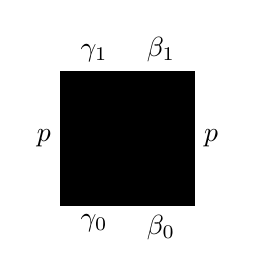
\begin{tikzpicture}[scale=.85]
		\draw[fill=\shadinga] (0, 0) rectangle (2, 2);
		\draw[dotted] (1, 0)--(1, 2);
		\draw (1.5,  0) node[below] {$\beta_0$};
		\draw (1.5,  2) node[above] {$\beta_1$};
		\draw (.5, 0) node[below] {$\gamma_0$};
		\draw (0, 1) node[left] {$p$};
		\draw (.5, 2) node[above] {$\gamma_1$};
		\draw (2,  1) node[right] {$p$};
		\draw (.5, 1) node {$H^\gamma_{01}$};
		\draw (1.5, 1) node {$H^\beta_{01}$};
		\end{tikzpicture}}a homotopy between  $\gamma_0\cdot \beta_0$ and $\gamma_1\cdot \beta_1$. Let $H^\gamma_{01}$ be the homotopy between the $\gamma_i$, and $H^\beta_{01}$ be the homotopy between the $\beta_i$. Define a new homotopy $H(x, t)$ be the piecewise composition:
	\[H(x, t)=\left\{ \begin{array}{cc} H^\gamma_{01}(2x, t) & x\in [0, 1/2]\\ H^\beta_{01} (2x-1, t) & x\in (1/2, 1]\end{array}\right.\]
	This homotopy can be visualized on the left as the associated composition of the homotopy domains. 

\end{proof}

\begin{claim}
	The composition rule is associative on homotopy equivalence classes of loops.
\end{claim}
\begin{proof}
	We need to exhibit the homotopy \[(\gamma_0\cdot \gamma_1)\cdot \gamma_2)\sim\gamma_0\cdot (\gamma_1\cdot \gamma_2)\] The difference between these two composition is only in the speeds which they trace out their respective paths.  The first composition goes through $\gamma_0$ and $\gamma_1$ at 4x speed,  and then $\gamma_2$ through double speed.   
	If we look at the second composition we instead draw $\gamma_0$ at double speed,  and $\gamma_1,  \gamma_2$ at 4x speed. \\
	In order to give a homotopy between these two composition, we merely need to reparameterize the domains to change drawing speed.\\
  Define the following homotopy between $(\gamma_0\cdot \gamma_1)\cdot \gamma_2)$ and $\gamma_0\cdot (\gamma_1\cdot \gamma_2)$. 
  \[H(x,  t)=\left\{\begin{array}{cc} 
                    	\gamma_0(4/(1+t) x) & x\in [0, (t+1)/4)\\
                    	\gamma_1(4(x-(1+t)/4))& x\in [(t+1)/4,  (t+2)/4)\\
                    	\gamma_2(4/(2-t)( x- (t+2)/4))& x\in [(t+2)/4,  1]
                    \end{array}\right.\]
	This homotopy is given by a really nasty function, and it is much easier 
\smarginnotel{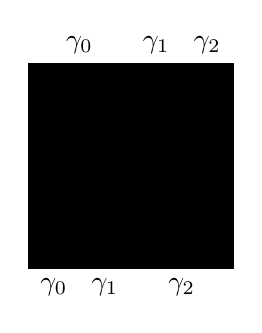
\begin{tikzpicture}[scale=1.3]
	\draw[fill=\shadinga] (0, 0) rectangle (2, 2);
	\draw[dashed] (1, 0)--(1.5, 2);
	\draw[dashed] (.5,  0)--(1,  2);
	\draw (.25, 0) node[below] {$\gamma_0$};
	\draw (.75, 0) node[below] {$\gamma_1$};
	\draw (1.5,  0) node[below] {$\gamma_2$};
	\draw (.5,  2) node[above] {$\gamma_0$};
	\draw (1.25,  2) node[above] {$\gamma_1$};
	\draw (1.75,  2) node[above] {$\gamma_2$};
\end{tikzpicture}}
	to see what this homotopy does by looking at the associated diagram of the domain. The bottom and top of the rectangle correspond to our two composition tracing out the loop $\gamma_0\cdot \gamma_1\cdot \gamma_2$ at different rates. . Each region of the rectangle corresponds to a constant homotopy between $\gamma_i$ and itself.  The diagonal stripe in the rectangle shows that there is a simple reparameterization of the domain that makes these compositions homotopic.
\end{proof}

\end{doubledtuftepage}
\begin{doubledtuftepage}[Making the Fundamental Group]
We'll now assemble the operation of loops into an algebraic object.  
	\begin{definition}
		Let the \emph{fundamental group} $(\pi_1(X, p), \cdot) $ be the set of homotopy classes of loops based at $p$ in $X$, with operation $\cdot$ given by loop composition. 
	\end{definition}
We already know that $\pi_1(X, p)$ has an associative product on it; the goal of this section is to prove that this is a group. 
\begin{claim}
	The constant loop $1_{x_0}$ has the property that
	\[[1_{x_0}]\cdot [\gamma]=[\gamma]\cdot [1_{x_0}]=[\gamma]\]
	for any loop $\gamma$ based at $x_0$. 
\end{claim}
\begin{proof}
	We use the fact that the constant loop can be reparameterized to any length that we choose. We define the homotopy as follows:
	\[
		H(x,  t)=\left\{\begin{array}{cc}
		                	x_0 & x\in [0, (1-t)/2)\\
		                	\gamma((2-t)(x-(1-t)/2)) & x\in [(1-t)/2,  1]
		                \end{array}\right.
	\]
	Again,  easier to represent with a picture. 
\smarginnotel{\begin{tikzpicture}[scale=1]
	\draw (0, 0) rectangle (2, 2);
	\draw[dotted] (1, 0)--(0, 2);
	\draw (1.5,  0) node[below] {$\gamma$};
	\draw (.5,  0) node[below] {$x_0$};
	\draw (1,  2) node[above] {$\gamma$};
	\draw[->] (-1, -1)--(-1, -.5) ;
	\draw[->] (-1, -1)--(-.5,-1);
	\draw (-1,  -.5) node[above] {$t$};
	\draw (-.5, -1) node[right] {$x$};
\end{tikzpicture}}

\end{proof}

\begin{claim}
	Suppose that $\gamma(t)$ is a loop. Define $\gamma^{-1}$ to be the loop $\gamma(-t)$. Then 
	\[[\gamma]\cdot[\gamma^{-1}]=[1_{x_0}]\]
\end{claim}
\begin{proof}
	We need to exhibit a homotopy from the loops $\gamma$ and $\gamma^{-1}$ to the constant loop. A formula for this homotopy is 
	\[
		H(x,  t)=\left\{\begin{array}{cc}
		                	\gamma(2x) & x\in [0,  (1-t)/2)\\
		                	\gamma(t) & x\in [(1-t)/2, (1+t)/2)\\
		                	\gamma(1-2x) & x\in  [(1+t)/2,  1]
		                \end{array}\right.
	\]
	Which is,  as usual ,  easier to visualize as a picture instead of a piecewise function. 
\smarginnotel{	\begin{tikzpicture}[scale=1]
	\draw (0, 0) rectangle (2, 2);
	\draw[dotted] (1, 0)--(0, 2);
	\draw (1.5,  0) node[below] {$\gamma^{-1}$};
	\draw (.5,  0) node[below] {$\gamma^{\;}$};
	\draw (1,  2) node[above] {$x_0$};
	\draw[dotted] (1, 0)--(2, 2);
	\draw[->] (-1, -1)--(-1, -.5) ;
	\draw[->] (-1, -1)--(-.5,-1);
	\draw (-1,  -.5) node[above] {$t$};
	\draw (-.5, -1) node[right] {$x$};
\end{tikzpicture}}

\end{proof}

The three claims that we made above prove that $\pi(X,  x_0)$ is a group. 
\begin{definition}
	Let $\beta$ be a path in $X$ connecting $x_0$ to $x_1$. Define the \emph{change of base point map} $F_\beta: \pi(X,  x_1)\to \pi(X,  x_0)$ as follows. Suppose that $\gamma$ is a path that has endpoints at $x_1$. Then let 
	\[F_\beta(\gamma):=(\beta\cdot \gamma\cdot \beta^{-1})\].
	This map is only dependent on the homotopy class of $h$. 
\end{definition}
\begin{claim}
	The change of base point map is a group homomorphism. 
\end{claim}
\begin{proof}
	We need to prove that the map preserves the group composition law. Here is a picture why!
	\vspace{4cm}
\end{proof}

\begin{claim}
	Suppose that $X$ is path connected. Let $x_0,  x_1\in X$ be two points in $X$. Then $\pi(X,  x_0)$ is isomorphic to $\pi(X,  x_1)$. 
\end{claim}
\begin{proof}
	Since $X$ is connected,  it is clear that there is path $\beta$ with endpoints $x_0$ and $x_1$. Check that the change of base point map is in fact an isomorphism of groups by composing it with the reverse change of base point map. 
\end{proof}

\end{doubledtuftepage}

\begin{claim}
	Suppose that $X$ and $Y$ are two different space,  and $f: X\to Y$ is a continuous function. Then there is an induced group homomorphism $f_*: \pi(X,  x_0)\to \pi(Y,  f(x_0))$. 
\end{claim}
\begin{proof}
	Using a function $f: X\to Y$,  we can take loops in $X$ and get loops in $Y$ as follows. Let $\gamma: [0, 1]\to X$ be a loop. Define 
	\[f_*(\gamma)=f\circ\gamma:[0, 1]\to Y.\]
	We can check that if $\gamma_0 \sim \gamma_1$,  then it is the case that $f_*(\gamma_0)\sim f_*(\gamma_1)$. This is because if $H(x,  t)$ is a homotopy between $\gamma_0$ and $\gamma_1$,  then $f(H(x,  t))$ is a homotopy between $f_*(\gamma_0)$ and $g_*(\gamma_1)$. \\
	Finally,  we need to check that $f_*$ respects the group operation,  that is 
	\[f_*(\gamma_0\circ \gamma_1)=f_*(\gamma_0)\circ f_*(\gamma_1)\]
\end{proof}

\begin{claim}
	Suppose that $f: X\to Y$ and $g: Y\to Z$ are two continuous maps. Then 
	\[g_*\circ f_*=(f\circ g)_*\]
\end{claim}



\begin{theorem}
	The fundamental group of the circle is $\Z$. 
\end{theorem}
\begin{proof}
	To come later in this class. But the idea is that the number of times that a loop winds around the origin tells you what number to map every loop to. 
\end{proof}

\subsection{Van Kampen's Theorem}
We would like a way to compute the fundamental group of a space $X=A\cup B$ in terms of its components $A$ and $B$. As with homology, we expect the fundamental group of this thing to be related to the fundamental group of their intersection. 
\begin{definition}
Let $G, H$ be two groups. The \emph{free product} of $G$ and $H$ is the unique group $G*H$ with maps $i:G\to G*H $, and $j: H\to G*H$ such that for any group $A$ and maps $f: G\to A$ and $g: H\to A$, there exists a unique map $\phi: G*H\to A$ such that the following diagram commutes:
\[
\begin{tikzcd}
G\arrow{d}{i} \arrow{dr}{f}\\  G*H \arrow[dashed]{r}{\phi} & A\\ H\arrow{u}{j} \arrow{ur}{h}
\end{tikzcd}
\]
\end{definition}

\begin{theorem}
Let $A$, $B$ be path connected topological spaced. Let $A\vee B$ be the \emph{wedge sum} of $A$ and $B$. Then $\pi_1(A\vee B)=\pi_1(A)*\pi_1(B).$
\end{theorem}

\section{Knot Group}
\subsection{Given as a Braid}
Here is one method for computing the fundamental group of the knot complement. Let $\beta$ be a braid which closes to $K$. Our intuition for computing the fundamental group of the knot complement will be as follows: first, think of the space $\S^3\setminus K$ as the union of two donuts where one donut contains the braid. Then cut this braid containing donut into a cylinder. Now, understand how the braid inside of the donut gives relations to the generators of the fundamental group of this cylinder. 
\[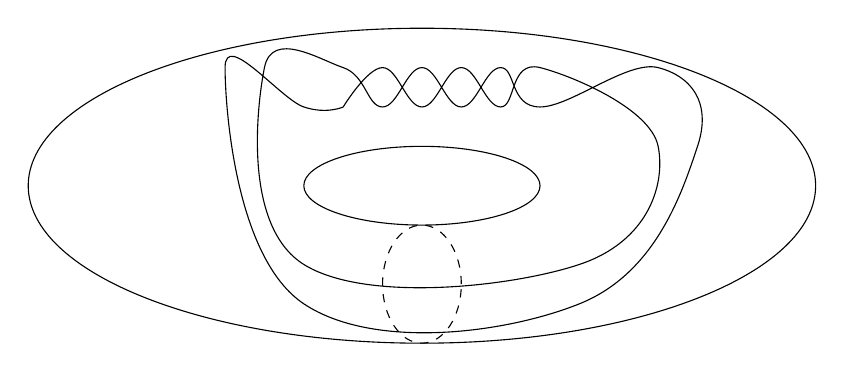
\begin{tikzpicture}[scale=.5]
\draw  plot[smooth, tension=.7] coordinates {(-3,2) (-2,3) (-1,2) (0,3) (1,2) (2,3) (5,1) (3,-2) (-4,-2) (-5,3) (-3,3) (-2,2) (-1,3) (0,2) (1,3) (2,2) (5,3) (6,1) (3,-3) (-4,-3) (-6,3) (-4,2) (-3,2)};
\draw  (-1,0) ellipse (3 and 1);
\draw  (-1,0) ellipse (10 and 4);
\draw[dashed]  (-1,-2.5) ellipse (1 and 1.5);
\end{tikzpicture}\]

Now, to make this idea rigorous, we use Van Kampen's theorem on the following decomposition. We work in cylindrical coordinates. Assume that the knot is from the closure of a braid $\beta$ on $n$ strings, and is given in such a way so that the orientation of the knot aligns with $\theta$ from our cylindrical coordinates. Furthermore, assume the whole knot is contained in the donut $(r-2)^2+z^2\leq 1$, and assume that the braid $\beta$ is contained in the portion of the torus $\theta\in [0, 180]$, so the remainder of the knot is just lines of constant $r, \theta$ values. Then we decompose the space into two parts:
\begin{itemize}
\item The first part $A$ of the space contains the braid (and a little strip for good luck.) This is the union of the cylinder $(0<\theta<2\pi, (r-1)^2+z^2<1$, and a small strip-- an open neighborhood of the curve $r=1, z=0$. Here is a drawing of the set $A$.
\[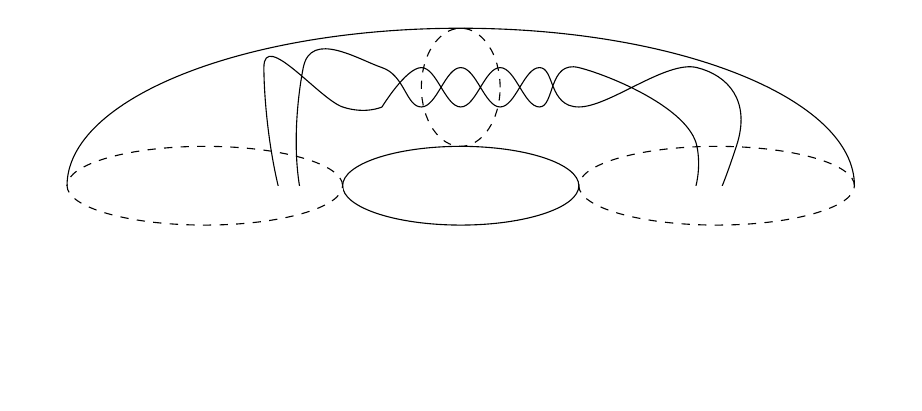
\begin{tikzpicture}[scale=.5]
\draw  plot[smooth, tension=.7] coordinates {(-3,2) (-2,3) (-1,2) (0,3) (1,2) (2,3) (5,1) (3,-2) (-4,-2) (-5,3) (-3,3) (-2,2) (-1,3) (0,2) (1,3) (2,2) (5,3) (6,1) (3,-3) (-4,-3) (-6,3) (-4,2) (-3,2)};
\draw  (-1,0) ellipse (3 and 1);
\draw  (-1,0) ellipse (10 and 4);
\draw[dashed]  (-1,+2.5) ellipse (1 and 1.5);
\fill[white]  (-12,0) rectangle (-4,-5);
\fill[white] (-6,-2) rectangle (5,-5);
\fill[white](2,0) rectangle (10
,-5);
\draw[dashed]  (-7.5,0) ellipse (3.5 and 1);
\draw[dashed]  (5.5,0) ellipse (3.5 and 1);
\end{tikzpicture}\]
\item The second part $B$ is a small open neighborhood of the complement of $A$.  This is a harder set to draw, so we will not do so here. 
\end{itemize}
Clearly from definition $A\cup B=S^3\setminus K$.  Now what does the intersection of $A$ and $B$ look like? It is a hollow cylinder, with $n$ holes poked in both the top and bottom, with a little handle attached to it. \\
Now why decompose the knot into each of these three space? Because their fundamental groups are so simple. 
\begin{itemize}
\item The Fundamental group of $A$ is the free group on $n+1$ generators, where the $+1$ generator is coming from the little handle added on.  Notice that since the braid has been ``unclosed'' it is homotopically the same as the cylinder missing $n$ lines, which has a fundamental group the free group generated by loops that go around each string complement.
\item The Fundamental group so $B$ is the free group on $n$ generators. 
\item The Fundamental group of $A\cap B$ is the Free group on $(2n-1)+1$ generators. The $2n$ generators correspond to the holes poked in the bottom and top of the hollow cylinder. The $-1$ corresponds to the fact that the loop that goes around all the generators on the left is equal to the loop that goes around all the generators on the right. The $+1$ corresponds to the lucky look that we have added on. 
\end{itemize}
Now clearly, the relationships from $B$ tell us that the left side generators of $A\cap B$ are equal to the right side generators of $A\cap B$. So, the fundamental group of $A\cup B$ will be given by generators of $A$ (less the special handle) mod out relations given by the braid, which we will write as $\beta(a)$. Now how does the braid effect these generators? \\
The braid acts by automorphism on the group $F^n=\pi_1(\R^2\setminus \{1, \ldots n\})$, by permuting the loops. In class, we proved that these automorphisms were given by 
\[\sigma_i(a_j)=\left\{\begin{array}{cc} a_j & j\neq i,i-1\\
a_j^{-1}a_{j+1}a_j & j=i\\
a_i+1 & j=i-1
\end{array}\right.
\]
\begin{example}
With the trefoil, we can use the braid word $\sigma_1^3$ which closes to the braid. The automorphisms that we get are that 
\begin{align*}
a_2=\sigma^{3}(a_2)=\sigma^2(a_1)\\
a_2=\sigma(a_1^{-1} a_2 a_1)\\
a_2=& a_1^{-1} a_2^{-1} a_1 a_1 a_1^{-1} a_2 a_1\\
a_1 a_2 a_1^{-1}= a_2^{-1} a_1 a_2
\end{align*}
These are the relations for the braid group! 
\end{example}
\subsection{Wirtinger Presentation}
The second way to compute the knot fundamental group is to do Van Kampen's theorem on every single crossing in the knot. Here is the idea for this method of computing the fundamental group.
\begin{itemize}
\item Using a planar diagram of the knot, make it so the arcs of the knot lie all in a place $z=0$, unless there is a crossing, where the string can pop up to a height of one.\\
\item Set a base point for computing the fundamental group at some negative $z$ value.\\
\item At each crossing, remove a small ball that contains the over and under crossings. \\
\[\begin{tikzpicture}

\draw  plot[smooth, tension=.7] coordinates {(-6,0) (4,0)};
\draw (-4,-3) -- (-2,-1) -- (-2,1) -- (0,3) -- (0,1) -- (3,4);
\draw  (-1,1) ellipse (4 and 4);
\node at (0,-5) {$x_0$};
\node at (-6,1) {$\alpha$};
\node at (-4,-4) {$\beta$};
\node at (4,1) {$\gamma$};
\node at (3,5) {$\delta$};
\end{tikzpicture}\]

\item Now we have a bunch of arcs connecting removed balls. Each arc gives a generator for the fundamental group.
\item Figure out what relations we add back in when we put in the balls. 
\end{itemize}
To figure out what relation we add back in, we just need to understand what the fundamental group of the sphere missing 4 points is related to the ball with two arcs removed is. If $\alpha, \beta, \gamma$ and $ \delta$ are the four loops on the boundary sphere, with base point at the bottom of the sphere, then the relation between them is given by $\alpha=\gamma^{-1}$, and $\beta=\alpha^{-1} \delta^{-1}\alpha$. This means that the added relations that we get at each crossing are that the ``through'' arc stays the same, but the under arcs are related by conjugation by the ``through'' arc. \project